\chapter{DESENVOLVIMENTO DO \textit{SOFTWARE}}

Tendo como destaque o código implementado, serão apresentados as principais funções desenvolvidas para cálculo dos indicadores de: variação de tensão; fator de potência; distorções harmônicas; desequilíbrio de tensão; flutuação de tensão e; variação de frequência.

O \autoref{cod:variacao_tensao} implementa a \autoref{eq:drp} e \autoref{eq:drc}, que determina os indicadores DRP e DRC. Esse função é chamada dentro de um \textit{loop} por 1008 vezes na classe ``Analysis".

\begin{codigo}
  \includecode[Python]{Código que calcula os indicadores de variação de tensão}{cod:variacao_tensao}{50}{illustrations/codes/voltage_variation.py}
\end{codigo}


Para determinação e análise do fator de potência foi desenvolvida a classe do \autoref{cod:power_factor}. Ela classifica o fator de potência em crítico e adequado a depender dos limites determinados pelo PRODIST.

\begin{codigo}
  \includecode[Python]{Classe para verificação do fator de potência}{cod:power_factor}{5}{illustrations/codes/power_factor.py}
\end{codigo}

A função principal da classe utilizada para determinar os indicadores de distorções harmônicas pode ser observada no \autoref{cod:harmonics}. Essa função percorre todos os harmônicos por meio de um \textit{loop for} para então determinar o indicador de acordo com as equações fornecidas pelo PRODIST.

O \autoref{cod:voltage_imbalance} foi desenvolvido para determinar o fator de desequilíbrio de tensão $FD$, por meio da aplicação da \autoref{eq:fd_2}.

\begin{codigo}
  \includecode[Python]{Função para cálculo dos indicadores de distorções harmônicas}{cod:harmonics}{16}{illustrations/codes/harmonics.py}
\end{codigo}

\begin{codigo}
  \includecode[Python]{Função para cálculo do fator de desequilíbrio de tensão}{cod:voltage_imbalance}{9}{illustrations/codes/voltage_imbalance.py}
\end{codigo}

Dentro da classe responsável pela análise de todos os indicadores foi criado uma função para determinação do indicador de flutuação de tensão, como pode ser observado no \autoref{cod:flicker}.

\begin{codigo}
  \includecode[Python]{Função para cálculo do indicador de flutuação de tensão}{cod:flicker}{140}{illustrations/codes/flicker.py}
\end{codigo}


Para aplicação da análise de variação de frequência, foi desenvolvido o \autoref{cod:frequency}. Ele classifica a frequência em adequada, baixa e alta, através de uma comparação com os níveis fornecidos pelo PRODIST.

\begin{codigo}
  \includecode[Python]{Função para análise da variação de frequência}{cod:frequency}{12}{illustrations/codes/frequency.py}
\end{codigo}

\chapter{RESULTADOS}

Nesse capítulo serão abordados os resultados obtidos com a utilização do código desenvolvido sendo alimentado dos dados colhidos pelo analisador de qualidade de energia.

\section{DEMONSTRAÇÃO DA INTERFACE GRÁFICA}

A \autoref{fig:tela_inicial} demonstra a visão geral da interface gráfica desenvolvida. Observa-se uma barra de seleção de arquivo, destacada na \autoref{fig:barra_selecao}, e utilizada para digitar o caminho referente a planilha de dados, um botão para abrir o gerenciador de arquivos do sistema operacional e um botão para carregar o arquivo quando selecionado.

\begin{figure}[H]
	\centering
	\caption{Tela inicial da interface gráfica}
	\label{fig:tela_inicial}
	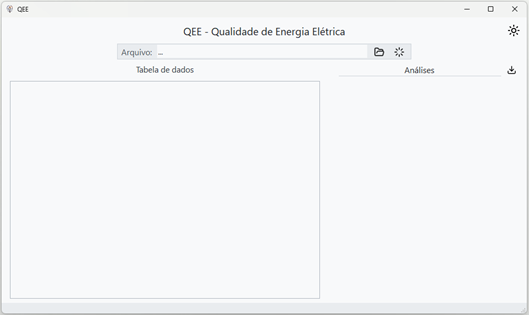
\includegraphics[width=15cm]{illustrations/figures/tela_inicial.png}
	\fonte{Autoria própria.}
\end{figure}

\begin{figure}[H]
	\centering
	\caption{Barra de seleção de arquivo}
	\label{fig:barra_selecao}
	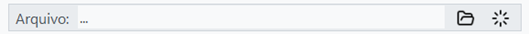
\includegraphics[width=15cm]{illustrations/figures/barra_selecao.png}
	\fonte{Autoria própria.}
\end{figure}

A interface contém mensagens informativas, para situações de inconsistência em valores fornecidos e confirmações de ações realizadas, como pode ser observado na \autoref{fig:mensagens_informativas}.

A \autoref{fig:moensagem_erro} mostra o exemplo para as mensagens de erros, enquanto \autoref{fig:moensagem_aviso} para mensagem de aviso e \autoref{fig:moensagem_informacao} para mensagens de informações.

\begin{figure}[H]
	\centering
	\caption{Mensagens informativas}
  \label{fig:mensagens_informativas}
	\begin{subfigure}{7.5cm}
		\centering
		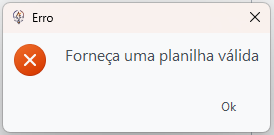
\includegraphics[height=3cm]{illustrations/figures/mensagem_erro.png}
		\caption{Mensagem de erro}
		\label{fig:moensagem_erro}
	\end{subfigure}
  \begin{subfigure}{7.5cm}
		\centering
		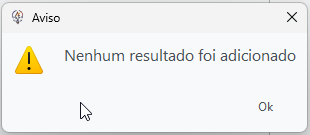
\includegraphics[height=3cm]{illustrations/figures/mensagem_aviso_resultado.png}
		\caption{Mensagem de aviso}
		\label{fig:moensagem_aviso}
	\end{subfigure}
  \begin{subfigure}{7.5cm}
		\centering
		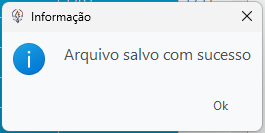
\includegraphics[height=3cm]{illustrations/figures/mensagem_informacao.png}
		\caption{Mensagem de informação}
		\label{fig:moensagem_informacao}
	\end{subfigure}
	\fonte{Autoria própria.}
\end{figure}

Quando for selecionada uma planilha adequada, aceita pela interface, os respectivos dados aparecem na tabela de dados, como mostrado na \autoref{fig:tabela_carregada}.

\begin{figure}[H]
  \centering
  \caption{Tabela de dados com os valores importados da planilha}
  \label{fig:tabela_carregada}
  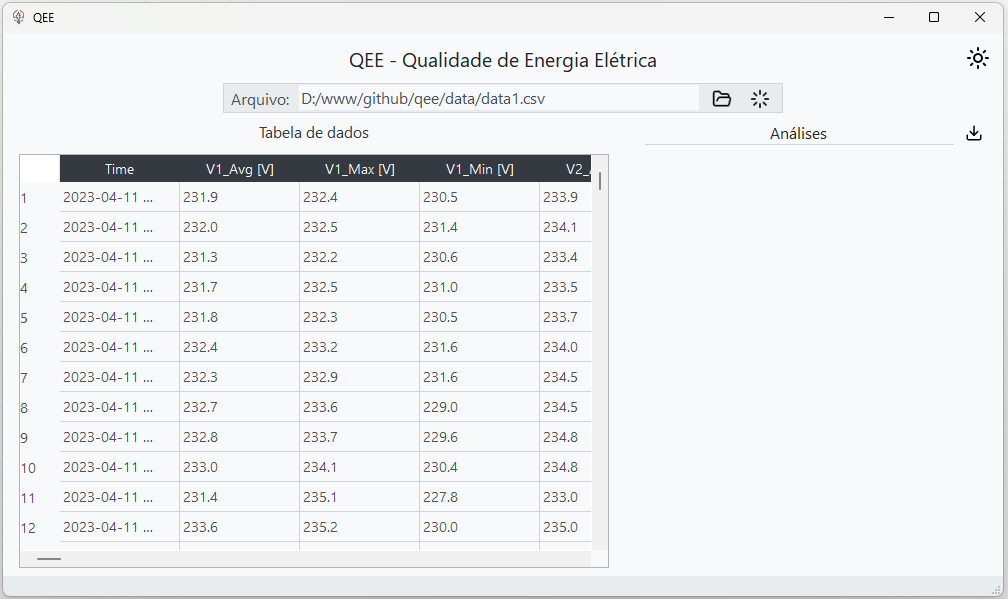
\includegraphics[width=15cm]{illustrations/figures/tabela_carregada.png}
  \fonte{Autoria própria.}
\end{figure}

A tabela da \autoref{fig:tabela_carregada} é a base para utilização da interface. Ao clicar sobre ela com o botão direito do \textit{mouse}, aparece um menu suspenso com as funções (Gerar gráfico, Variação de tensão, Fator de potência, Distorções harmônicas, Desequilíbrio de tensão, Flutuação de tensão e Variação de frequência), como mostra a \autoref{fig:menu_suspenso}.

\begin{figure}[H]
  \centering
  \caption{Menu suspenso com as funções do \textit{software}}
  \label{fig:menu_suspenso}
  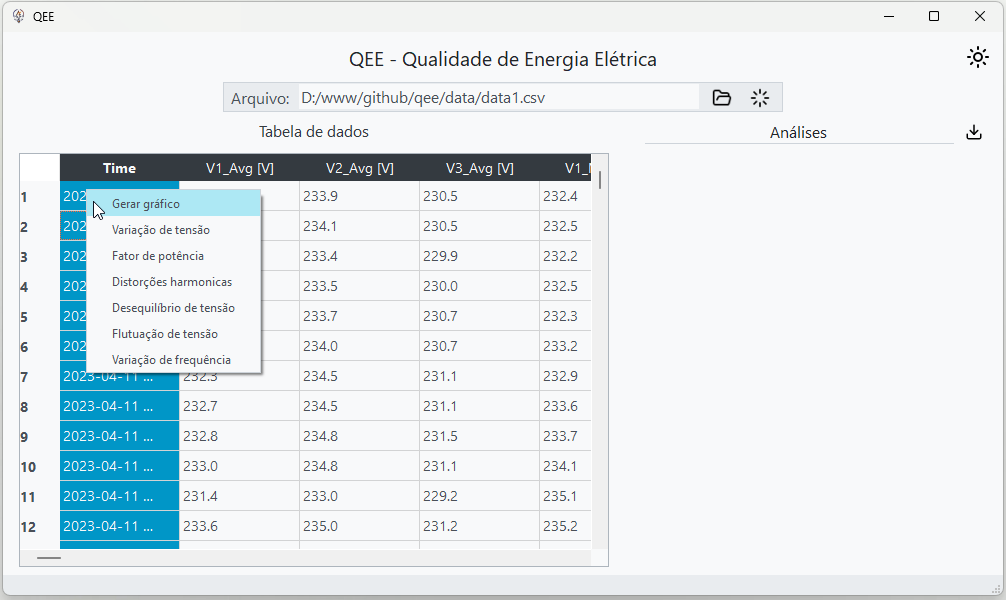
\includegraphics[width=15cm]{illustrations/figures/menu_suspenso.png}
  \fonte{Autoria própria.}
\end{figure}

\subsection{Gerar gráfico}

Nessa função é possível visualizar um gráfico contendo uma classificação das tensões em adequada, precária ou crítica. Ao clicar na função “Gerar gráfico”, sobre um parâmetro de tensão dentro da tabela, aparecerá uma caixa de seleção de nível de tensão (\autoref{fig:selecao_niveis_tensao}) para seleção da tensão de referência a qual a interface utiliza para verificar a classificação dos níveis de tensões.

\begin{figure}[H]
  \centering
  \caption{Caixa de seleção de nível de tensão}
  \label{fig:selecao_niveis_tensao}
  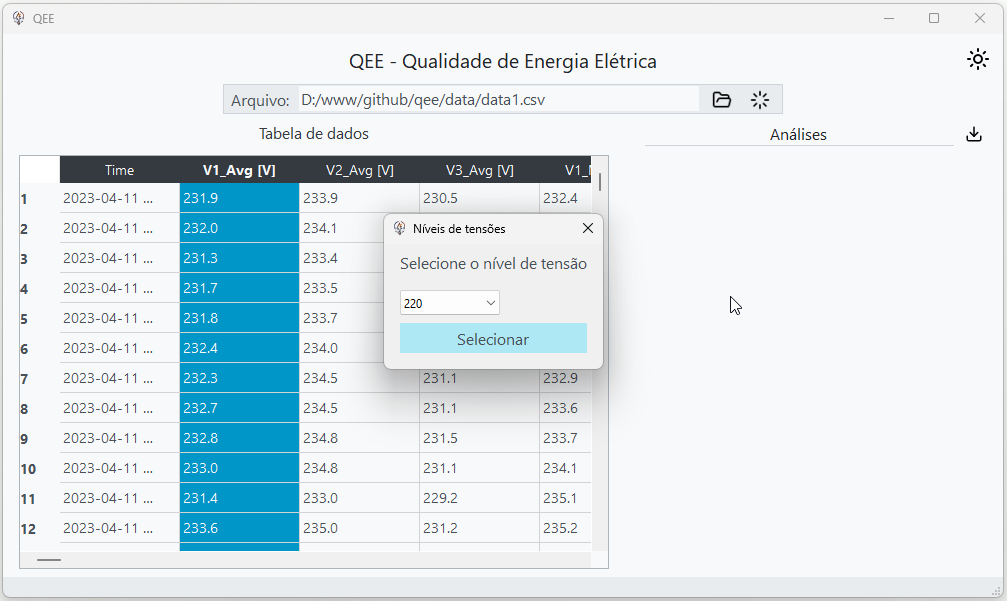
\includegraphics[width=15cm]{illustrations/figures/selecao_niveis_tensao.png}
  \fonte{Autoria própria.}
\end{figure}

Na \autoref{fig:grafico_tensao} é mostrada uma janela com o gráfico gerado ao selecionar o nível de tensão, no qual as demarcações para tensão adequada, precária e crítica, correspondem as cores da \autoref{fig:faixa_tensao}. Nessa janela também é possível editar e salvar o gráfico.

\begin{figure}[H]
  \centering
  \caption{Gráfico com a classificação dos níveis de tensão}
  \label{fig:grafico_tensao}
  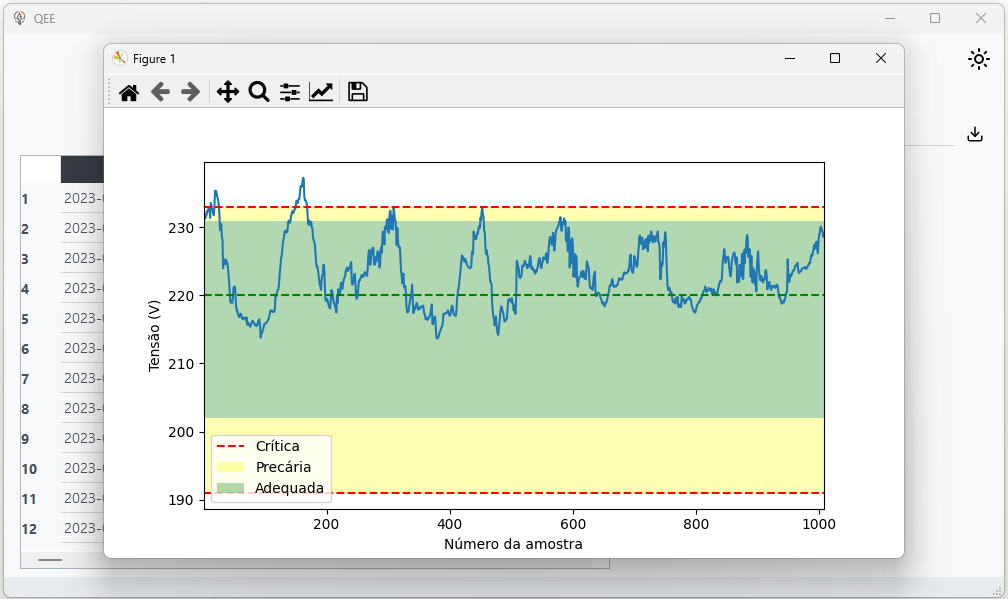
\includegraphics[width=15cm]{illustrations/figures/grafico_tensao.png}
  \fonte{Autoria própria.}
\end{figure}

\subsection{Variação de tensão}

Para uma análise dos valores de tensões demonstrado na \autoref{fig:grafico_tensao}, o PRODIST determina os indicadores de variação de tensão DRP e DRC. Partindo disso, a função seguinte da interface é a “Variação de tensão”, em que o usuário precisa selecionar os 3 níveis de tensão, seja tensões de fase ou tensões de linha, como mostrado na \autoref{fig:selecao_niveis_tensao_valores}.

\begin{figure}[H]
  \centering
  \caption{Seleção dos níveis de tensão}
  \label{fig:selecao_niveis_tensao_valores}
  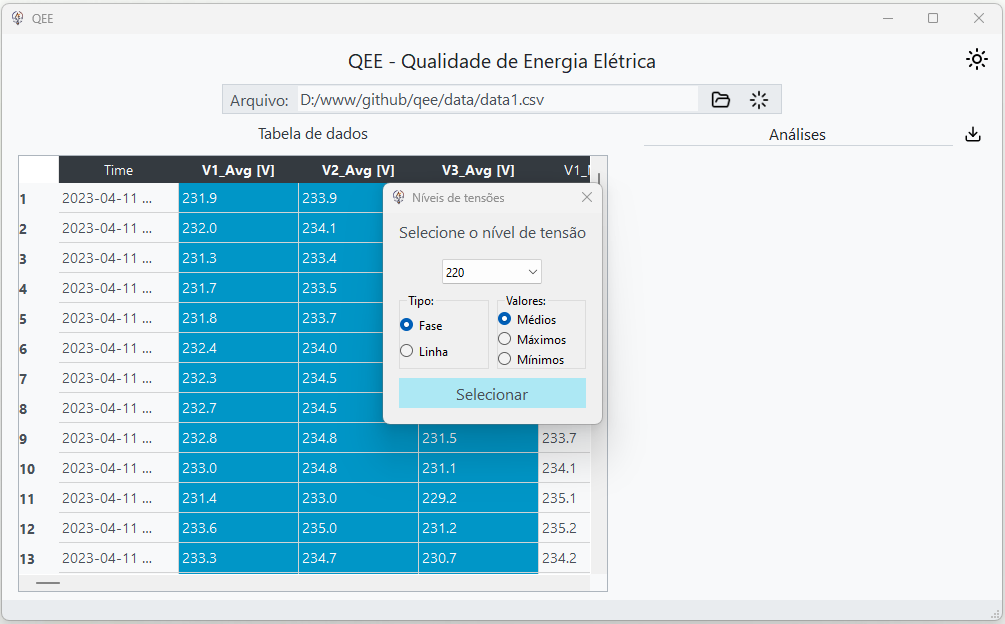
\includegraphics[width=15cm]{illustrations/figures/selecao_niveis_tensao_valores.png}
  \fonte{Autoria própria.}
\end{figure}

Na barra ``Análises", à direita da interface na \autoref{fig:exemplo_variacao_tensao}, aparece uma lista com as análises que já foram feitas, possuindo, além disso, as funções de remover e salvar um resultado específico, ou salvar toda a análise.

\begin{figure}[H]
  \centering
  \caption{Resultado do cálculo dos indicadores de variação de tensão}
  \label{fig:exemplo_variacao_tensao}
  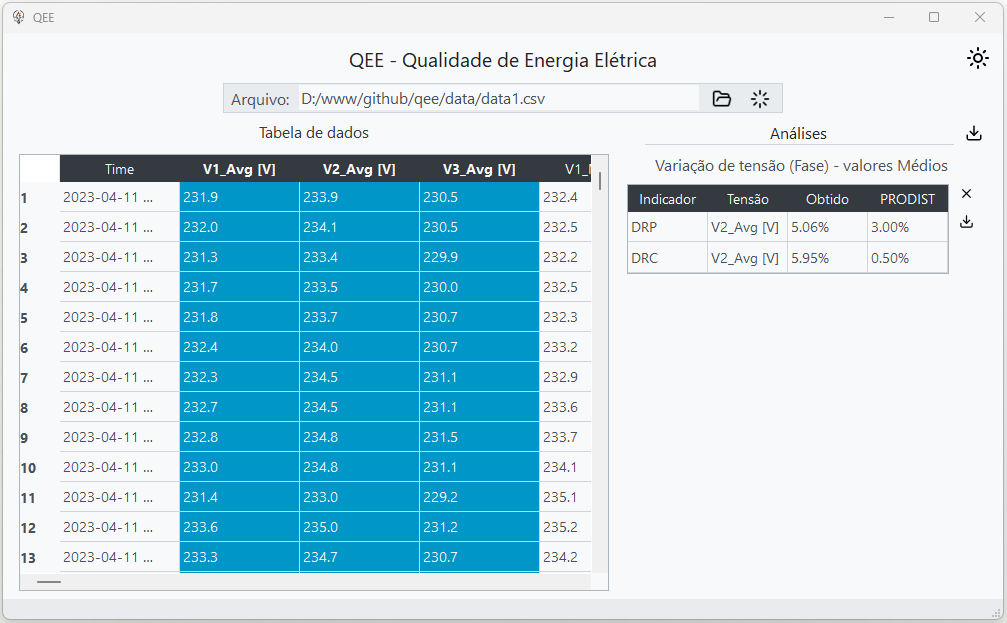
\includegraphics[width=15cm]{illustrations/figures/exemplo_variacao_tensao.png}
  \fonte{Autoria própria.}
\end{figure}

\subsection{Fator de potência}

A função “Fator de potência” analisa o fator de potência, classificando em situação crítica quando abaixo de 0,92 e adequado para maior ou igual, como mostra \autoref{fig:exemplo_fator_potencia}.

\begin{figure}[H]
  \centering
  \caption{Análise do fator de potência}
  \label{fig:exemplo_fator_potencia}
  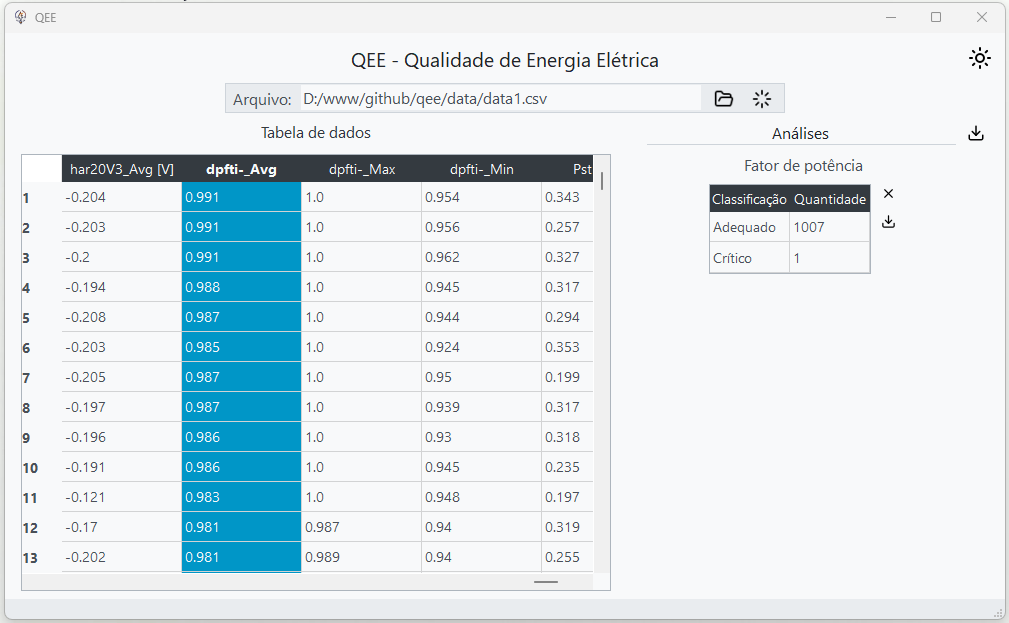
\includegraphics[width=15cm]{illustrations/figures/exemplo_fator_potencia.png}
  \fonte{Autoria própria.}
\end{figure}

\subsection{Distorções harmônicas}

Já a função “Distorções harmônicas” calcula os indicadores de distorções harmônicas, como mostra a \autoref{fig:exemplo_dh}.


\begin{figure}[H]
  \centering
  \caption{Cálculo dos indicadores de distorções harmônicas}
  \label{fig:exemplo_dh}
  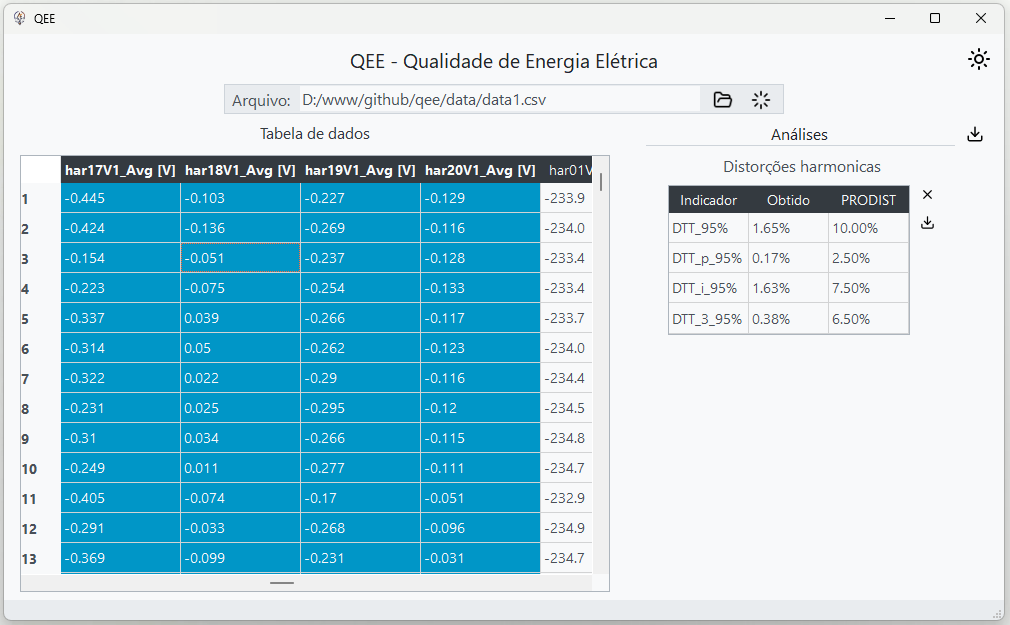
\includegraphics[width=15cm]{illustrations/figures/exemplo_dh.png}
  \fonte{Autoria própria.}
\end{figure}

\subsection{Desequilíbrio de tensão}

Para a função de desequilíbrio de tensão é necessário selecionar as três tensões de linha. Sendo assim o \textit{software} calcula o indicador, como mostra a \autoref{fig:exemplo_dt}

\begin{figure}[H]
  \centering
  \caption{Cálculo do indicador de desequilíbrio de tensão}
  \label{fig:exemplo_dt}
  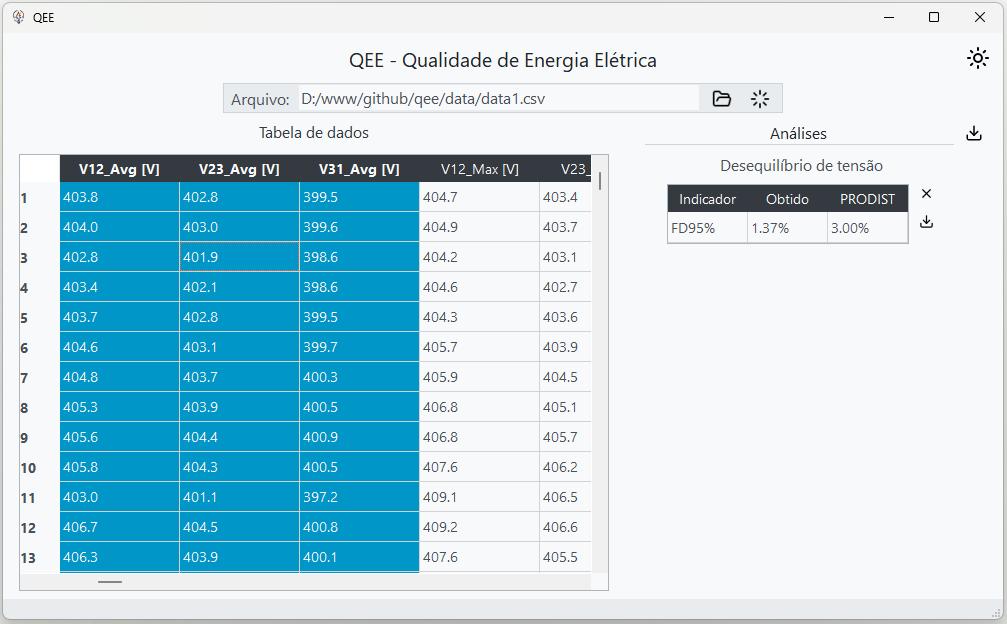
\includegraphics[width=15cm]{illustrations/figures/exemplo_dt.png}
  \fonte{Autoria própria.}
\end{figure}

\subsection{Flutuação de tensão}

A função ``Flutuação de tensão'' determina o indicador $P_{st}95\%$, \autoref{fig:exemplo_ft}.

\begin{figure}[H]
  \centering
  \caption{Cálculo do indicador de flutuação de tensão}
  \label{fig:exemplo_ft}
  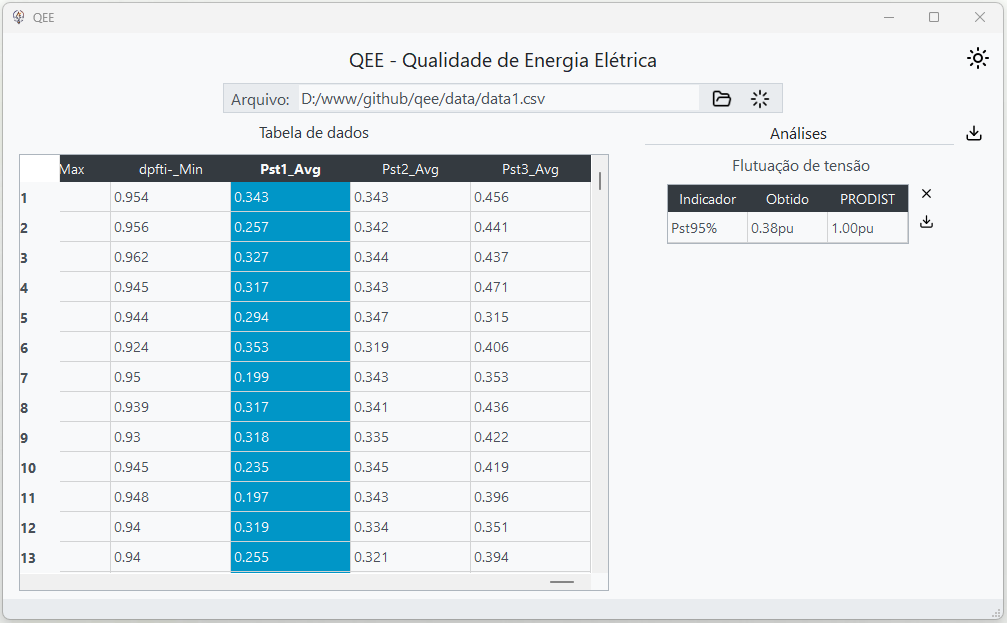
\includegraphics[width=15cm]{illustrations/figures/exemplo_ft.png}
  \fonte{Autoria própria.}
\end{figure}

\subsection{Variação de frequência}

“Variação de frequência” é a última função da interface. Ela expressa a classificação da frequência em alta, adequada e baixa (\autoref{fig:exemplo_vf}).

\begin{figure}[H]
  \centering
  \caption{Análise da variação de frequência}
  \label{fig:exemplo_vf}
  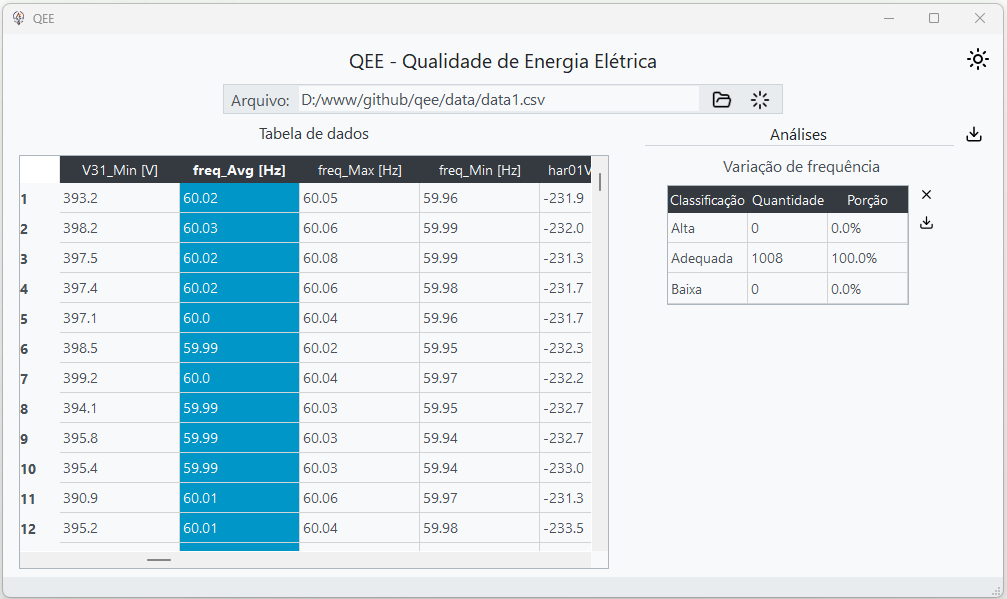
\includegraphics[width=15cm]{illustrations/figures/exemplo_vf.png}
  \fonte{Autoria própria.}
\end{figure}

\section{ANÁLISE DOS DADOS}

Todos os resultados expostos nessa seção foram obtidos através da utilização de duas amostras de dados, coletadas pelo mesmo analisador de dados e dispostos nos Apêndices desse trabalho. Sendo:

\begin{itemize}
  \item \autoref{ap:graficos_a1} - gráficos das tensões com classificação - amostra 1, referente aos dados colhidos da medição no bloco dos professores I;
  \item \autoref{ap:graficos_a2} - gráficos das tensões com classificação - amostra 2, para os dados colhidos da medição na usina fotovoltaica;
  \item \autoref{ap:analise_a1} - relatório de análise de QEE gerado pela rotina computacional - amostra 1;
  \item \autoref{ap:analise_a2} - relatório de análise de QEE gerado pela rotina computacional -
  amostra 2;
\end{itemize}

\subsection{Variação de tensão}

Nessa etapa foram efetuadas análises para as tensões de fase e linha, nais quais foram determinados os indicadores DRP e DRC para as duas amostras injetadas no \textit{software}.

Os indicadores para tensão de fase foram dispostos na \autoref{tab:vt_fase_a1} e \autoref{tab:vt_fase_a2}.

\begin{table}[H]
  \centering
  \caption{Indicadores de variação de tensão de fase para amostra 1}
  \label{tab:vt_fase_a1}
  \begin{tabular}{@{}ccccc@{}}
    \toprule
   \textbf{Indicador} & \textbf{Médios (\%)} & \textbf{Máximos (\%)} & \textbf{Mínimos (\%)} & \textbf{PRODIST (\%)} \\
    \midrule
    $DRP$ & $5,06$ & $7,74$ & $3,57$ & $3,00\%$ \\
    $DRC$ & $5,95$ & $10,12$ & $1,88$ & $0,50\%$ \\
    \bottomrule
  \end{tabular}
  \fonte{Autoria própria.}
\end{table}

\begin{table}[H]
  \centering
  \caption{Indicadores de variação de tensão de fase para amostra 2}
  \label{tab:vt_fase_a2}
  \begin{tabular}{@{}ccccc@{}}
    \toprule
   \textbf{Indicador} & \textbf{Médios (\%)} & \textbf{Máximos (\%)} & \textbf{Mínimos (\%)} & \textbf{PRODIST (\%)} \\
    \midrule
    $DRP$ & $0,20$ & $1,98$ & $0,30$ & $3,00\%$ \\
    $DRC$ & $0,20$ & $0,60$ & $0,20$ & $0,50\%$ \\
    \bottomrule
  \end{tabular}
  \fonte{Autoria própria.}
\end{table}

Analisando essas duas amostras pode se notar que apenas a amostra 2 (\autoref{tab:vt_fase_a2}) está dentro dos limites determinados pelo PRODIST. 

De maneira análoga as tensões de fase, foram determinados os indicadores para tensões de linha conforme \autoref{tab:vt_linha_a1} e \ref{tab:vt_linha_a2}.

\begin{table}[H]
  \centering
  \caption{Indicadores de variação de tensão de linha para amostra 1}
  \label{tab:vt_linha_a1}
  \begin{tabular}{@{}ccccc@{}}
    \toprule
   \textbf{Indicador} & \textbf{Médios (\%)} & \textbf{Máximos (\%)} & \textbf{Mínimos (\%)} & \textbf{PRODIST (\%)} \\
    \midrule
    $DRP$ & $10,42$ & $8,93$ & $4,66$ & $3,00\%$ \\
    $DRC$ & $11,01$ & $6,35$ & $3,08$ & $0,50\%$ \\
    \bottomrule
  \end{tabular}
  \fonte{Autoria própria.}
\end{table}

\begin{table}[H]
  \centering
  \caption{Indicadores de variação de tensão de linha para amostra 2}
  \label{tab:vt_linha_a2}
  \begin{tabular}{@{}ccccc@{}}
    \toprule
    \textbf{Indicador} & \textbf{Médios (\%)} & \textbf{Máximos (\%)} & \textbf{Mínimos (\%)} & \textbf{PRODIST (\%)} \\
    \midrule
    $DRP$ & $0,69$ & $2,78$ & $0,40$ & $3,00\%$ \\
    $DRC$ & $0,20$ & $0,60$ & $0,20$ & $0,50\%$ \\
    \bottomrule
  \end{tabular}
  \fonte{Autoria própria.}
\end{table}

Ao comparar essas duas amostras, nota-se que a amostra 1 não está dentro dos limites enquanto que a amostra 2 está, com a exceção do indicador $DRC$ para valores Máximos.

\subsection{Fator de potência}

Para o fator de potência a única amostra utilizada consistiu na amostra 1, isso porque a amostra 2 correspondia a uma medição antiga que não possuía os valores de fator de potência. Determinando assim a classificação conforme \autoref{tab:fp_amostra1}.

\begin{table}[H]
  \centering
  \caption{Classificação do fator de potência para amostra 1}
  \label{tab:fp_amostra1}
  \begin{tabular}{@{}cccc@{}}
    \toprule
    Classificação & Médios & Máximos & Mínimos \\
    \midrule
    Adequado & 1007 & 1007 & 911 \\
    Crítico & 1 & 1 & 97 \\
    \bottomrule
  \end{tabular}
  \fonte{Autoria própria.}
\end{table}

Os valores médios, máximos e mínimos dispostos na \autoref{tab:fp_amostra1}, representam a quantidade de leituras para esses valores que ficaram dentro do intervalo determinado pelo PRODIST (Adequado) e fora (Crítico).

\subsection{Distorções harmônicas}

Os indicadores de distorções harmônicas encontrados para amostra 1 e amostra 2 foram dispostos na \autoref{tab:dh_amostra1} e \autoref{tab:dh_amostra2}, respectivamente, em que $V_1$, $V_2$ e $V_3$ são as tensões referentes aos harmônicos.

\begin{table}[H]
  \centering
  \caption{Indicadores de distorções harmônicas para amostra 1}
  \label{tab:dh_amostra1}
  \begin{tabular}{@{}ccccc@{}}
    \toprule
    \textbf{Indicador} & \textbf{$V_1$ (\%)} & \textbf{$V_2$ (\%)} & \textbf{$V_3$ (\%)} & \textbf{PRODIST  (\%)} \\
    \midrule
    $DTT95\%$   & 1,65 & 1,83 & 1,80 & 10,00 \\
    $DTT_p95\%$ & 0,17 & 0,19 & 0,18 & 2,50 \\
    $DTT_i95\%$ & 1,63 & 1,80 & 1,70 & 7,50 \\
    $DTT_395\%$ & 0,38 & 0,52 & 0,71 & 6,50 \\
    \bottomrule
  \end{tabular}
  \fonte{Autoria própria.}
\end{table}

\begin{table}[H]
  \centering
  \caption{Indicadores de distorções harmônicas para amostra 2}
  \label{tab:dh_amostra2}
  \begin{tabular}{@{}ccccc@{}}
    \toprule
    \textbf{Indicador} & \textbf{$V_1$ (\%)} & \textbf{$V_2$ (\%)} & \textbf{$V_3$ (\%)} & \textbf{PRODIST  (\%)} \\
    \midrule
    $DTT95\%$   & 1,85 & 2,08 & 39,70 & 10,00 \\
    $DTT_p95\%$ & 0,04 & 0,03 & 0,51 & 2,50 \\
    $DTT_i95\%$ & 1,84 & 2,03 & 34,79 & 7,50 \\
    $DTT_395\%$ & 0,53 & 0,64 & 20,14 & 6,50 \\
    \bottomrule
  \end{tabular}
  \fonte{Autoria própria.}
\end{table}

Observa-se, em ambos os casos, que os valores estão dentro do estabelecido pelo PRODIST.

\subsection{Desequilíbrio de tensão}

A \autoref{tab:fd_amostra1} contém os fatores de desequilíbrio de tensão calculados para os valores médios, máximos e mínimos das tensões de linha da amostra 1.

\begin{table}[H]
  \centering
  \caption{Fatores de desequilíbrio de tensão para amostra 1}
  \label{tab:fd_amostra1}
  \begin{tabular}{@{}ccccc@{}}
    \toprule
   \textbf{Indicador} & \textbf{Médios (\%)} & \textbf{Máximos (\%)} & \textbf{Mínimos (\%)} & \textbf{PRODIST (\%)} \\
    \midrule
    $FD95\%$  & 1,37 & 1,35 & 1,41 & 3,00 \\
    \bottomrule
  \end{tabular}
  \fonte{Autoria própria.}
\end{table}

Para amostra 2 os indicadores podem ser observados na \autoref{tab:fd_amostra2}.

\begin{table}[H]
  \centering
  \caption{Fatores de desequilíbrio de tensão para amostra 2}
  \label{tab:fd_amostra2}
  \begin{tabular}{@{}ccccc@{}}
    \toprule
   \textbf{Indicador} & \textbf{Médios (\%)} & \textbf{Máximos (\%)} & \textbf{Mínimos (\%)} & \textbf{PRODIST (\%)} \\
    \midrule
    $FD95\%$  & 1,11 & 1,11 & 1,15 & 3,00 \\
    \bottomrule
  \end{tabular}
  \fonte{Autoria própria.}
\end{table}

Mais uma vez, em ambos os casos, os indicadores estão dentro dos limites estabelecidos pelo PRODIST.

\subsection{Flutuação de tensão}

Para esse indicador, foram encontrados valores para as três tensões, como mostram a \autoref{tab:ft_amostra1} e \autoref{tab:ft_amostra2}.

\begin{table}[H]
  \centering
  \caption{Indicadores de flutuação de tensão para amostra 1}
  \label{tab:ft_amostra1}
  \begin{tabular}{@{}ccccc@{}}
    \toprule
    Indicador & V1 (pu) & V2 (pu) & V3 (pu) & PRODIST  (pu) \\
    \midrule
    $P_{st}95\%$   & 0,38 & 0,84 & 0,43 & 1,00 \\
    \bottomrule
  \end{tabular}
  \fonte{Autoria própria.}
\end{table}

\begin{table}[H]
  \centering
  \caption{Indicadores de flutuação de tensão para amostra 2}
  \label{tab:ft_amostra2}
  \begin{tabular}{@{}ccccc@{}}
    \toprule
    Indicador & V1 (pu) & V2 (pu) & V3 (pu) & PRODIST  (pu) \\
    \midrule
    $P_{st}95\%$   & 0,26 & 0,28 & 0,30 & 1,00 \\
    \bottomrule
  \end{tabular}
  \fonte{Autoria própria.}
\end{table}

Novamente, tanto no primeiro quanto no segundo caso, os indicadores permanecem dentro dos parâmetros estipulados pelo PRODIST.

\subsection{Variação de frequência}

A amostra 1 obteve as classificações apresentadas na \autoref{tab:vf_amostra1}, em que os valores médios, máximos e mínimos, correspondem as porções percentuais do total de amostras para cada classificação.

\begin{table}[H]
  \centering
  \caption{Classificação da variação de frequência para amostra 1}
  \label{tab:vf_amostra1}
  \begin{tabular}{@{}cccc@{}}
    \toprule
    Classificação & Médios (\%) & Máximos (\%) & Mínimos (\%) \\
    \midrule
    Alta & 0,00 & 0,60 & 0,00 \\
    Adequada & 100,00 & 99,40 & 99,70 \\
    Baixa & 0,00 & 0,00 & 0,30 \\
    \bottomrule
  \end{tabular}
  \fonte{Autoria própria.}
\end{table}

A \autoref{tab:vf_amostra2} contém a classificação da variação de frequência para amostra 2.

\begin{table}[H]
  \centering
  \caption{Classificação da variação de frequência para amostra 2}
  \label{tab:vf_amostra2}
  \begin{tabular}{@{}cccc@{}}
    \toprule
    Classificação & Médios (\%) & Máximos (\%) & Mínimos (\%) \\
    \midrule
    Alta & 0,00 & 0,99 & 0,00 \\
    Adequada & 100,00 & 99,01 & 99,01 \\
    Baixa & 0,00 & 0,00 & 0,99 \\
    \bottomrule
  \end{tabular}
  \fonte{Autoria própria.}
\end{table}

Nos dois cenários, observa-se que a maioria das classificações de frequências se enquadram em situação adequada, com um pequeno percentual inferior a 1\%, seja para alta ou baixa, fora disso.
